\section{Implementation of the Lind Prototype}
\label{sec.implementation}

Based on the design in Section \ref{sec.design},
we implemented a secure sandbox system, Lind,
for running untrusted user programs in vulnerable OS kernels.
Lind adopts two basic technologies as its building blocks\textendash
%Google's Native Client (NaCl), and Seattle's Repy.
%
%As described in Figure \ref{fig:design} and Section 4.2, our design has
%two main components\textendash a computation module that isolates the
%application and a library OS module that isolates the complex
%portions of POSIX, a standard OS interface Lind provides. We choose 
Google's Native Client (NaCl)~\cite{NaCl-09} as the computation
module for efficient execution of legacy code in the
form of x86 and ARM binaries, and 
Seattle's Repy~\cite{Repy-10} as the library OS. 
%(Figure \ref{fig:architecture}), since it is a restricted subset of Python,
%that works as a sandbox to provide a safer environment to run untrusted code.

%\begin{figure}%[h]
%\centering
%	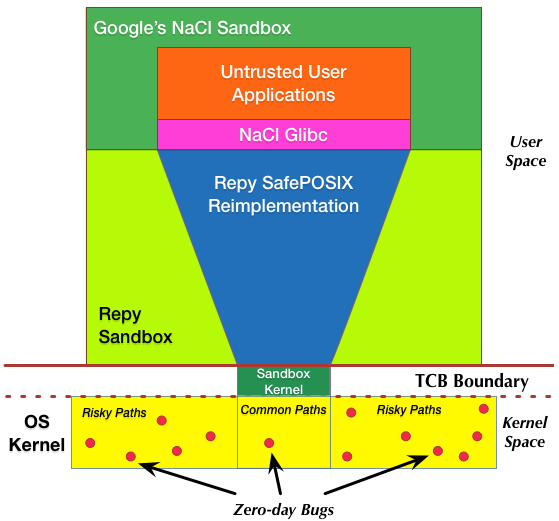
\includegraphics[width=1.0\columnwidth]{diagram/lind_architecture_new.png}
%	\caption{Architecture of Lind including various components such as NaCl, NaCl glibc, and Repy Sandbox.
%	User level applications will issue system calls that are dispatched through the Repy OS connector that bridges the Lind system to the OS Kernel.}
%\label{fig:architecture}
%\end{figure}

\subsection{Native Client}

We use NaCl to isolate the computation of the user application
from the kernel.
NaCl allows Lind to work on most types of legacy code.
It compiles the programs to produce a binary with software fault isolation.
This prevents the majority of the application from performing system calls
or executing arbitrary instructions.
%
To perform a system call, the application will call into a small privileged
part of the NaCl TCB that forwards system calls, usually to the OS for
processing. To build Lind, we changed the NaCl TCP to
forward these calls to our library OS that we call SafePOSIX 
for processing. 
% the following doesn't say anything new
%The NaCl glibc module contains stubs that reject operations
%that Chrome would not handle.  We added functionality to NaCl's glibc so that
%those calls could be forwarded into SafePOSIX for processing.

%NaCl can perform the functions required by the computation module well, and it is easy to
%connect with our system API module because NaCl uses glibc to perform system calls.
%Modification to NaCl's glibc would allow us to redirect those system call requests to our own system API module.
%
%NaCl is a sandbox used to execute untrusted x86 native code.
%It aims to give applications the computational performance of native applications without compromising safety.
%NaCl uses software fault isolation and a secure runtime to direct system interaction and
%side effects through interfaces managed by the program. It provides operating system portability
%for binary code while supporting performance-oriented features, such as thread support,
%instruction set extensions, such as SSE, and use of compiler intrinsics and a hand-coded assembler.
%It also allows the efficient execution of legacy code in the form of x86 and ARM binaries
%that are built with a lightly modified compiler tool chain.

\subsection{Seattle's Repy}

To build an API to access the safe parts of the underlying kernel, we need
two things.  First, we need a restricted sandbox that isolates computation
and only allows access to commonly used kernel paths.  We used
Seattle's Repy~\cite{Repy-10} sandbox to perform this task.
Second, we need to build a POSIX implementation to run within that sandbox.

%pplications. For Lind, we used Repy to build our system API module.
%To be more specific, our system API module has a very small sandbox kernel
%as TCB,  written with Python. On top of the sandbox kernel,
%we use Repy code to safely reimplement complex system functions.

\textbf{The Repy Sandbox Kernel.}
A natural concern with any sandbox design is that bugs are simply pushed into
another part of the trusted code base.  As it is the only piece of code added
to the system call paths of the TCB, the sandbox kernel's security is of
paramount concern. 
%The sandbox kernel needs to be secure and bug-free.
%Because it is the TCB of the system, any bugs in it could cause fatal problems.
%and allow attackers to access the OS kernel and gain kernel privilege.
We used Seattle's Repy system API due to its tiny sandbox kernel
(comprised of around 8K LOC), and is written to provide straightforward 
access to the minimal set of the system call API needed to build general 
computational functionality. Repy allows
%fit our key design principle that our proposed system should 
access only to the safe portions of the OS kernel with 33 basic API 
functions, including 13 network functions, 6 file functions, 6 threading functions,
and 8 miscellaneous functions~\cite{Repy-10, RepyKernel}. The code is 
written using style guidelines designed to ease security auditing
 of the code~\cite{style}. Most of these functions are simple and
regularly used system calls that access the commonly used kernel paths.

%\begin{table}
%\centering
%\caption {Repy sandbox kernel capabilities that supports NaCl functions, such as networking, file I/O operations and threading.}
%
%  \begin{tabular}{ | p{2.5cm} | p{4.5cm} |}
%  \hline
%  \textbf{Repy Function} & \textbf{Available System Calls}  \\ \hline
%
%Networking & \emph{gethostbyname, openconnection, getmyip, socket.send, socket.receive, socket.close,
%listenforconnection, tcpserversocket.getconnection, tcpserversocket.close, sendmessage, listenformessage,
%udpserversocket.getmessage, and udpserversocket.close.} \\ \hline
%
%I/O Operations & \emph{openfile, file.close, file.readat, file.writeat, listfiles, and removefile.} \\ \hline
%
%Threading & \emph{createlock, sleep, lock.acquire, lock.release, createthread, and getthreadname.} \\ \hline
%
%Miscellaneous Functions & \emph{getruntime, randombytes, log, exitall, createvirtualnamespace,
%virtualnamespace.evaluate, getresources, and getlasterror.}  \\ \hline
%    \end{tabular}
%    \label{table:RepyKernel}
%\end{table}

%\begin{table}
%\centering
%\scriptsize
%\caption {System Functions in the Repy Sandbox Kernel.  \cappos{Need to
%clearly explain the takeaway.}}
%\begin{tabular}{|l|}
%  \hline
% \textbf{Network Functions} \\
%  \hline
%  gethostbyname(name) \\
%  \hline
%  getmyip() \\
%  \hline
%  openconnection(destip, destport, localip, localport, timeout) \\
%  \hline
%  socket.close() \\
%  \hline
%  socket.recv(numbytes) \\
%  \hline
%  socket.send(message) \\
%  \hline
%  listenforconnection(localip, localport) \\
%  \hline
%  tcpserversocket.getconnection() \\
%  \hline
%  tcpserversocket.close()\\
%  \hline
%  sendmessage(destip, destport, message, localip, localport) \\
%  \hline
%  listenformessage(localip, localport) \\
%  \hline
%  udpserversocket.getmessage() \\
%  \hline
%  udpserversocket.close() \\
%  \hline \hline
%  \textbf{File Functions} \\
%  \hline
%  openfile(filename, create) \\
%  \hline
%  file.close() \\
%  \hline
%  file.readat(sizelimit, offset) \\
%  \hline
% file.writeat(data, offset) \\
%  \hline
%  listfiles() \\
%  \hline
%  removefile(filename) \\
%  \hline \hline
%  \textbf{Threading Functions} \\
%  \hline
%  createlock() \\
%  \hline
%  lock.acquire(blocking) \\
%  \hline
%  lock.release() \\
%  \hline
%  createthread(function) \\
 % \hline
 % sleep(seconds) \\
  %\hline
  %getthreadname() \\
  %\hline \hline
  %\textbf{Miscellaneous Functions} \\
  %\hline
 % getruntime() \\
  %\hline
 % randombytes() \\
  %\hline
  %log(*args) \\
  %\hline
  %exitall() \\
  %\hline
  %createvirtualnamespace(code, name) \\
  %\hline
  %virtualnamespace.evaluate(context) \\
  %\hline
  %getresources() \\
  %\hline
  %getlasterror() \\
  %\hline
%\end{tabular}
%\label{table:RepyKernel}
%\end{table}


The Repy kernel code has been
audited by a professional penetration tester.  Since 2010, there has also been
a bug bounty program for security flaws in the sandbox.
The code is deployed in daily use across thousands of devices,
including on the Seattle testbed \cite{seattle}, and has been examined by
hundreds of parties.  Developers have reported
XXX issues for problems in other parts of the systems. However, to date
no security flaws have been found in the sandbox kernel.
This does not provide any strong guarantees that bugs do not exist, and if
they do, the security of the system could be compromised.
However, having a small, easily auditable piece of code helps to reduce the
risk of such occurrence.

\textbf{The SafePOSIX Reimplementation.}
The key responsibility of our system API module is to serve system call requests from user code.
In Lind, those system call requests are issued from the user code,
received by NaCl, and then redirected to our system API module.
The API module includes a POSIX API to serve those requests.

A POSIX API is a set of standard operating system interfaces that provide operating system functions
to the user code. However, the POSIX API is large and complex enough that it is
very hard to ensure that its implementation is secure and bug-free.
%
%Our choice to use Repy helped us solve this architectural security problem.
Since Repy is a programming language sandbox, it can provide the ideal isolation
we needed when constructing our POSIX API. In Lind,
complex system functions are reimplemented using Repy code,
based on the ``safe-reimplement'' principle from our design in Section~{\ref{sec.design}}.

\subsection{Operations}

Lind combines NaCl and Repy to provide native computation and
safe access to the system. Untrusted programs are run in NaCl,
but access to all system resources is diverted to a Repy program.\yanyan{SafePOSIX?}
%This program is responsible for accessing the system on behalf of the Lind library
% OS. A NaCl sandbox is built on top of the Repy sandbox.
%
To service a system call in NaCl, a server routine marshals its arguments into a text string,
and sends the call and the arguments to the Repy sandbox.
The library OS then executes the appropriate system call, marshals the result and
returns it back to NaCl. The result is eventually returned as the appropriate native type to the calling program.

%Lind is designed to minimize the need to modify either sandbox. This is possible
%because the TCB of both were extremely small, and because the Lind code is run
%in both.
%\lois{Another odd sentence Yiwen and I discussed. I thought I knew how to
%fix it, but it still does not make sense. I would delete it.}

The only complex part of Lind is the library OS, which runs in Repy.
However, because Python is a very powerful language that provides rich functions,
it helps to make the construction of Lind easier. The downside of Python is that
some consider the language ``slow'',
because it is dynamically typed rather than statically typed, it is interpreted rather than compiled,
and Python's object model can lead to inefficient memory access.
Nevertheless, the internals of an application in Lind are run in NaCl, a very high performance
environment.

%This balances the performance of the system, with the ease of implementation and maintenance of the library OS component of Lind.\yanyan{I think this paragraph can be cut.}

%Lind is portable.
%Programs running inside Lind are using a standard POSIX glibc interface,
%and, since the Lind runtime is strictly user-level, it can work on many different platforms
%including Linux, Mac OS X and Windows.

The lightweight and minimized overhead is another feature of Lind. Because the sandbox only
 incurs overhead when there is a system call, overall overhead for Lind is low.
 Yet, it does not sacrifice performance for cost.
Lind uses a native interface for execution,
allowing CPU-and-memory-intensive applications to run at speeds that are equivalent
 to NaCl and near native speed.

In Section \ref{sec.evaluation}}, we report how the dual sandboxes and other elements
of Lind performed when compared with other virtualization systems.
